%
% Complete documentation on the extended LaTeX markup used for Insight
% documentation is available in ``Documenting Insight'', which is part
% of the standard documentation for Insight.  It may be found online
% at:
%
%     http://www.itk.org/

\documentclass{InsightArticle}

\usepackage[dvips]{graphicx}



%%%%%%%%%%%%%%%%%%%%%%%%%%%%%%%%%%%%%%%%%%%%%%%%%%%%%%%%%%%%%%%%%%
%
%  hyperref should be the last package to be loaded.
%
%%%%%%%%%%%%%%%%%%%%%%%%%%%%%%%%%%%%%%%%%%%%%%%%%%%%%%%%%%%%%%%%%%
\usepackage[dvips,
bookmarks,
bookmarksopen,
backref,
colorlinks,linkcolor={blue},citecolor={blue},urlcolor={blue},
]{hyperref}

\usepackage{url}


%  This is a template for Papers to the Insight Journal. 
%  It is comparable to a technical report format.

% The title should be descriptive enough for people to be able to find
% the relevant document.
\title{CTest Integration of Sikuli Automated GUI Testing}

% 
% NOTE: This is the last number of the "handle" URL that 
% The Insight Journal assigns to your paper as part of the
% submission process. Please replace the number "1338" with
% the actual handle number that you get assigned.
%
\newcommand{\IJhandlerIDnumber}{3196}

% Increment the release number whenever significant changes are made.
% The author and/or editor can define 'significant' however they like.
\release{0.00}

% At minimum, give your name and an email address.  You can include a
% snail-mail address if you like.
\author{Evan Schwab, Lydie Souhait, Nicolas Rannou, Kishore Mosaliganti\\
Arnaud Gelas, Sean Megason}
\authoraddress{Harvard Medical School, Megason lab}

\begin{document}

% Add hyperlink to the web location and license of the paper.
\IJhandlefooter{\IJhandlerIDnumber}


\ifpdf
\else
   %
   % Commands for including Graphics when using latex
   %
   \DeclareGraphicsExtensions{.eps,.jpg,.gif,.tiff,.bmp,.png}
   \DeclareGraphicsRule{.jpg}{eps}{.jpg.bb}{`convert #1 eps:-}
   \DeclareGraphicsRule{.gif}{eps}{.gif.bb}{`convert #1 eps:-}
   \DeclareGraphicsRule{.tiff}{eps}{.tiff.bb}{`convert #1 eps:-}
   \DeclareGraphicsRule{.bmp}{eps}{.bmp.bb}{`convert #1 eps:-}
   \DeclareGraphicsRule{.png}{eps}{.png.bb}{`convert #1 eps:-}
\fi

\maketitle

\ifhtml
\chapter*{Front Matter\label{front}}
\fi

\begin{abstract}
\noindent
\end{abstract}

\IJhandlenote{\IJhandlerIDnumber}

\tableofcontents
% ------------------------------------------------------------------------
\section{Introduction}

% ------------------------------------------------------------------------
\section{Sikuli}

% Feel free to change section titles
\subsection{What is sikuli?}

Sikuli~\cite{Sikuli:Documentation,Sikuli:Website,Yeh:2009:Sikuli} is a visual
technology to automate and test graphical user interfaces (GUI) using images
(screenshots). Sikuli includes \emph{Sikuli Script} and \emph{Sikuli IDE}.\\

\emph{Sikuli Script} automates anything you see on the screen without internal
API's support. Sikuli Script is a programming language that uses screen shot
images as variables and objects in order to automate graphical user interface
functions. The Sikuli Script is built on a Jython (Python for Java platform)
library which uses Python syntax in addition to a number of special Sikuli
functions for acquiring and handling screen shot images and performing mouse,
keyboard actions.\\

In the \emph{Sikuli IDE}, the user can write scripts that include screen shot
thumbnails so they can visually track the functions of their code. The most
useful functions from Sikuli scripts are conveniently found as
buttons on the IDE. When using the IDE, Sikuli then saves a script in a
directory with a unique extension .sikuli. The directory consists of a python
script file (script file to be used by sikuli), an html file, and a list of all
the screenshot images used in the script.


\subsection{Simple Sikuli example} % not related to gofigure...

\begin{figure}[htp]
 \centering
 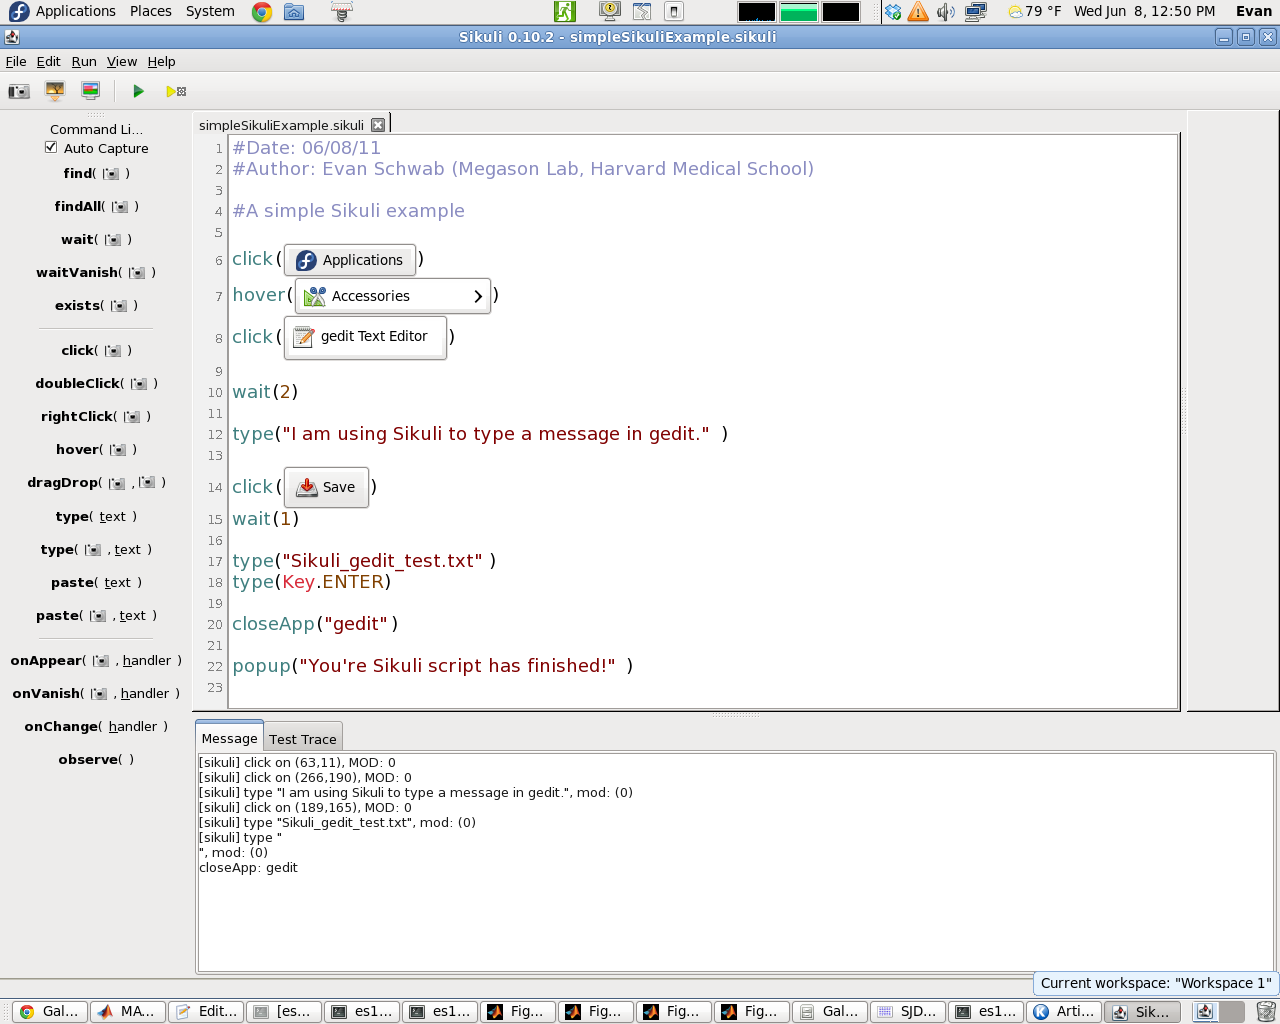
\includegraphics[width=0.99\textwidth]{./SimpleSikuliExample.png}
 % SimpleSikuliExample.png: 1280x1024 pixel, 72dpi, 45.16x36.12 cm, bb=0 0 1280 1024
 \caption{here is my caption}
 \label{fig:SimpleExample}
\end{figure}

% ------------------------------------------------------------------------
\section{Integration with CTest}
% I'll write it this part
One of Sikuli's primary uses is the automation of GUI testing for software
developers.  For GUI testing, it is useful to compartmentalize different software functions and test each unit
individually.  The newest versions of Sikuli come equipped with a Unit Testing feature 
Unit Testing.  Unit Testing can be called using the IDE or by command
line and enables the user to write multiple functions in a script which are
run individually.  At the end of the run, the Sikuli output will tell the user
how many tests ran successfully and which ones failed and where.  To connect this
Unit Testing feature directly to our software, we integrated Sikuli with CTest.
.....
.....


% ------------------------------------------------------------------------
\section{Example}
\begin{figure}[htp]
 \centering
 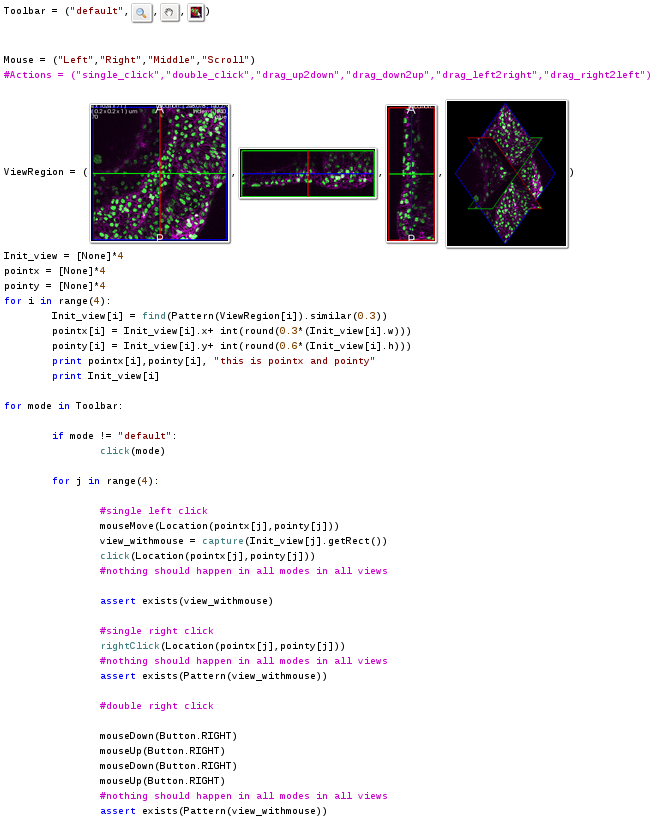
\includegraphics[width=0.99\textwidth]{./Gofigure2Example.png}
 % Gofigure2Example.png: 667x826 pixel, 72dpi, 23.53x29.14 cm, bb=0 0 667 826
 \caption{here is my caption}
 \label{fig:Gofigure2Example}
\end{figure}
% ------------------------------------------------------------------------
\section{Conclusion}

\clearpage

\bibliographystyle{plain}
\bibliography{InsightJournal,biblio}


\end{document}

